%%%%%%%%%%%%%%%%%%%%%%%%%%%%%%%%%%%%%%%%%%%%%%%%%%%%%%%%
\documentclass[12pt,a4paper]{article}% 文档格式
\usepackage{ctex,hyperref}% 输出汉字
\usepackage{times}% 英文使用Times New Roman
%%%%%%%%%%%%%%%%%%%%%%%%%%%%%%%%%%%%%%%%%%%%%%%%%%%%%%%%
\title{\fontsize{18pt}{27pt}\selectfont% 小四字号,1.5倍行距
{\heiti% 黑体
计算物理——针对LCG的一点思考}}% 题目
%%%%%%%%%%%%%%%%%%%%%%%%%%%%%%%%%%%%%%%%%%%%%%%%%%%%%%%%
\author{\fontsize{12pt}{18pt}\selectfont% 小四字号,1.5倍行距
{\fangsong% 仿宋
白博臣}\\% 标题栏脚注
\fontsize{10.5pt}{15.75pt}\selectfont% 五号字号,1.5倍行距
{\fangsong% 仿宋
(四川大学~~~物理学拔尖计划)}}% 作者单位,“~”表示空格
%%%%%%%%%%%%%%%%%%%%%%%%%%%%%%%%%%%%%%%%%%%%%%%%%%%%%%%%
\date{}% 日期(这里避免生成日期)
%%%%%%%%%%%%%%%%%%%%%%%%%%%%%%%%%%%%%%%%%%%%%%%%%%%%%%%%
\usepackage{amsmath,amsfonts,amssymb}% 为公式输入创造条件的宏包
%%%%%%%%%%%%%%%%%%%%%%%%%%%%%%%%%%%%%%%%%%%%%%%%%%%%%%%%
\usepackage{graphicx}% 图片插入宏包
\usepackage{subfigure}% 并排子图
\usepackage{float}% 浮动环境,用于调整图片位置
\usepackage[export]{adjustbox}% 防止过宽的图片
%%%%%%%%%%%%%%%%%%%%%%%%%%%%%%%%%%%%%%%%%%%%%%%%%%%%%%%%
\usepackage{bibentry}
\usepackage{natbib}% 以上2个为参考文献宏包
%%%%%%%%%%%%%%%%%%%%%%%%%%%%%%%%%%%%%%%%%%%%%%%%%%%%%%%%
\usepackage{abstract}% 两栏文档,一栏摘要及关键字宏包
\renewcommand{\abstracttextfont}{\fangsong}% 摘要内容字体为仿宋
\renewcommand{\abstractname}{\textbf{摘\quad 要}}% 更改摘要二字的样式
%%%%%%%%%%%%%%%%%%%%%%%%%%%%%%%%%%%%%%%%%%%%%%%%%%%%%%%%
\usepackage{xcolor}% 字体颜色宏包
\newcommand{\red}[1]{\textcolor[rgb]{1.00,0.00,0.00}{#1}}
\newcommand{\blue}[1]{\textcolor[rgb]{0.00,0.00,1.00}{#1}}
\newcommand{\green}[1]{\textcolor[rgb]{0.00,1.00,0.00}{#1}}
\newcommand{\darkblue}[1]
{\textcolor[rgb]{0.00,0.00,0.50}{#1}}
\newcommand{\darkgreen}[1]
{\textcolor[rgb]{0.00,0.37,0.00}{#1}}
\newcommand{\darkred}[1]{\textcolor[rgb]{0.60,0.00,0.00}{#1}}
\newcommand{\brown}[1]{\textcolor[rgb]{0.50,0.30,0.00}{#1}}
\newcommand{\purple}[1]{\textcolor[rgb]{0.50,0.00,0.50}{#1}}% 为使用方便而编辑的新指令
%%%%%%%%%%%%%%%%%%%%%%%%%%%%%%%%%%%%%%%%%%%%%%%%%%%%%%%%
\usepackage{url}% 超链接
\usepackage{bm}% 加粗部分公式
\usepackage{multirow}
\usepackage{booktabs}
\usepackage{epstopdf}
\usepackage{epsfig}
\usepackage{longtable}% 长表格
\usepackage{supertabular}% 跨页表格
\usepackage{algorithm}
\usepackage{algorithmic}
\usepackage{changepage}% 换页
%%%%%%%%%%%%%%%%%%%%%%%%%%%%%%%%%%%%%%%%%%%%%%%%%%%%%%%%
\usepackage{enumerate}% 短编号
\usepackage{caption}% 设置标题
\captionsetup[figure]{name=\fontsize{10pt}{15pt}\selectfont Figure}% 设置图片编号头
\captionsetup[table]{name=\fontsize{10pt}{15pt}\selectfont Table}% 设置表格编号头
%%%%%%%%%%%%%%%%%%%%%%%%%%%%%%%%%%%%%%%%%%%%%%%%%%%%%%%%
\usepackage{indentfirst}% 中文首行缩进
\usepackage[left=2.50cm,right=2.50cm,top=2.80cm,bottom=2.50cm]{geometry}% 页边距设置
\renewcommand{\baselinestretch}{1.5}% 定义行间距(1.5)
%%%%%%%%%%%%%%%%%%%%%%%%%%%%%%%%%%%%%%%%%%%%%%%%%%%%%%%%
\usepackage{fancyhdr} %设置全文页眉、页脚的格式
\pagestyle{fancy}
\hypersetup{colorlinks=true,linkcolor=black}% 去除引用红框,改变颜色


%%%%%%%%%%%%%%%%%%%%%%%%%%%%%%%%%%%%%%%%%%%%%%%%%%%%%%%%
\newtheorem{theorem}{\indent 定理}[section]
\newtheorem{lemma}[theorem]{\indent 引理}
\newtheorem{proposition}[theorem]{\indent 命题}
\newtheorem{corollary}[theorem]{\indent 推论}
\newtheorem{definition}{\indent 定义}[section]
\newtheorem{example}{\indent 例}[section]
\newtheorem{remark}{\indent 注}[section]
\newenvironment{solution}{\begin{proof}[\indent\bf 解]}{\end{proof}}
\renewcommand{\proofname}{\indent\bf 证明}

%%%%%%%%%%%%%%%%%%%%%%%%%%%%%%%%%%%%%%%%%%%%%%%%%%%%%%%%

\begin{document}% 以下为正文内容
    \maketitle% 产生标题,没有它无法显示标题
    %%%%%%%%%%%%%%%%%%%%%%%%%%%%%%%%%%%%%%%%%%%%%%%%%%%%%%%%
    \lhead{}% 页眉左边设为空
    \chead{}% 页眉中间设为空
    \rhead{}% 页眉右边设为空
    \lfoot{}% 页脚左边设为空
    \cfoot{\thepage}% 页脚中间显示页码
    \rfoot{}% 页脚右边设为空
    %%%%%%%%%%%%%%%%%%%%%%%%%%%%%%%%%%%%%%%%%%%%%%%%%%%%%%%%
    \begin{abstract}
        \fangsong
        本文探讨了线性同余发生器(LCG)的特性及其在随机数生成中的应用。LCG是一种利用求余运算的简单随机数生成器,其递推公式为$x_n = (ax_{n-1}+c) \pmod{M}$,其中M是模数,a是乘数,c是增量,$x_0$是初始种子。LCG产生的序列$\{x_n\}$为非负整数,通过将$\{x_n\}$除以M得到的$\{R_n\}$可作为均匀随机数序列。

        在对LCG进行分析的过程中,作者发现了两个问题:首先,对于参数为$m=2^{31}-1,a=4,c=1$的LCG,初始种子值对最终收敛值有显著影响;其次,对于参数为$m=27,a=26,c=5$的LCG,不同的初始种子值会导致收敛值稳定在两个不同的值。这一发现挑战了随机数生成器应具有的期望值与种子值无关的特性。

        为了解释这些现象,作者从数学角度对LCG的特性进行了深入分析,并提出了通项公式$x_{n+1}=a^n(x_0+\frac{c}{a-1})-\frac{c}{a-1}$,以期找到问题的解答。


    \end{abstract}

    \begin{adjustwidth}{1.06cm}{1.06cm}
        \fontsize{10.5pt}{15.75pt}\selectfont{\heiti{关键词:}\fangsong{
            线性同余发生器,随机数生成,收敛性,数学分析
        }}\\
    \end{adjustwidth}

%    \begin{center}% 居中处理
%    {\textbf{Abstract}}% 英文摘要
%    \end{center}
%    \begin{adjustwidth}{1.06cm}{1.06cm}% 英文摘要内容
%        \hspace{1.5em}Attention!If you input "dif{}ferent", the computer will output "different", but if you input "dif\{\}ferent", the computer will output "dif{}ferent"
%    \end{adjustwidth}
    \newpage% 从新的一页继续


    \section{LCG简介}
    LCG(Linear congruential generator)即线性同余发生器,是利用求余运算的随机数发生器。其递推公式为:
    \begin{equation}
        \begin{split}
            x_n = (ax_{n-1}+c) & \pmod{M}, \quad n=1,2,\ldots \\
            m\text{为模数;} & 0<m \\
            a\text{为乘数;} & 0\leq a < m \\
            c\text{为增量;} & 0\leq c < m \\
            x_{0}\text{为初始种子;} & 0\leq x_0 <m
        \end{split}\label{eq:equation}
    \end{equation}
    得到的序列${x_n}$为非负整数,$0\leq x_n \leq M$。最后令$R_n=x_n/M$,则$R_n\in [0,1)$,把${R_n}$作为均匀随机数序列。
    该算法的基本思想是因为很大的整数前面的位数是重要的有效位数 而后面若干位有一定随机性。
    因为线性同余法的递推算法仅依赖于前一项,序列元素取值只有$M$个可能取值,所以产生的序列$x_0,x_1,x_2,\ldots$一定会重复。若存在正整数$n$和$m$使得$x_n=x_m(m<n)$,则必有
    $x_{n+k}=x_{m+k},k=0,1,2,\ldots$即$x_n,x_{n+1},x_{n+2},\ldots$重复了$x_m,x_{m+1},x_{m+2},\ldots$,称这样的$n-m$的最小值$T$为此随机数发生器在初值$x_0$下的周期,易得,$T\leq M$.


    \section{问题发现}
    本课程EX12要求复现PPT中的某个图像(Figure 1):

    \begin{figure}[htbp]
        \centering
        \includegraphics[height=8cm]{PPT}
        \caption{EX12要求复现四组参数值下LCG的期望收敛性}\label{fig:figure}
    \end{figure}

    在复现过程中,发现两个奇怪的现象:

    1.针对图像中参数为$m=2^{31}-1,a=4,c=1$的折线,我们发现初始值(种子值)对折线最后的收敛值有影响。

    2.针对图像中参数为$m=27,a=26,c=5$的折线,我们发现其收敛值根据种子值的不同最后稳定在两个值。

    现对两个问题进行进一步阐述。

    \subsection{问题一阐述}
    当选取种子值$x_0=1$时,我们可以得到Figure 2,而当我们更改种子值为$x_0=12345678$时,得到的图像为Figure 3.

    \begin{figure}[H]% 插入两张图片并且并排
        \centering
        \begin{minipage}{0.48\textwidth}
            \centering
            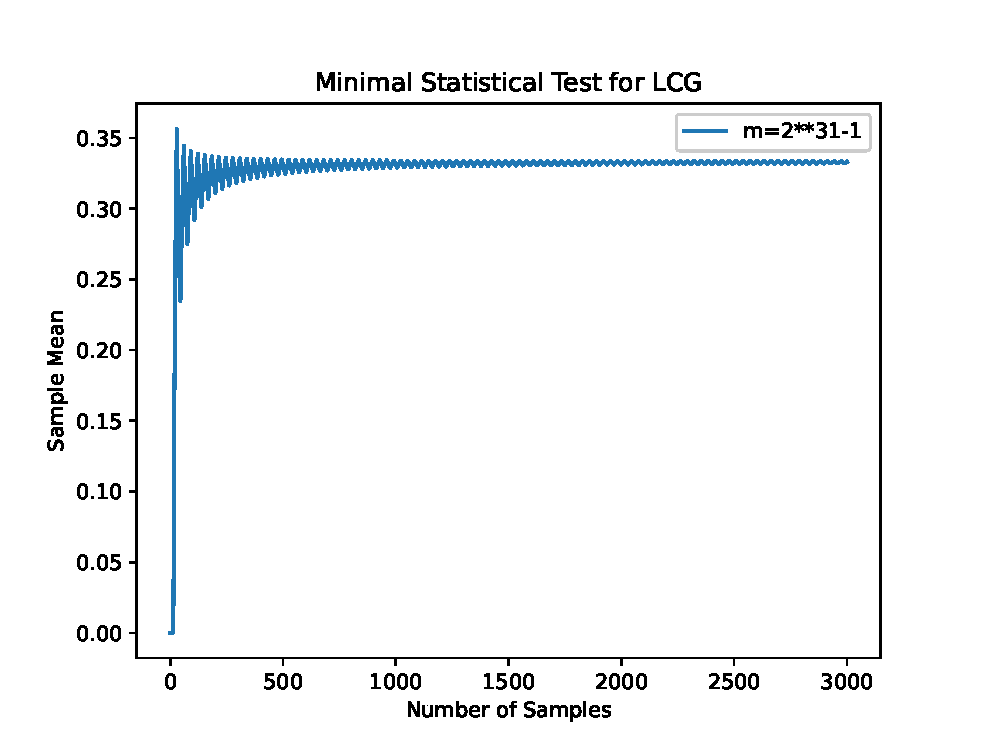
\includegraphics[width=1.1\textwidth]{Problem_1}
            \caption{\fontsize{10pt}{15pt}\selectfont 种子值取1时,最后并没有收敛到0.5,而是在0.3$\sim$ 0.35之间}
        \end{minipage}
        \hspace{0cm}% 图片间距
        \hfill% 撑满整行
        \begin{minipage}{0.48\textwidth}
            \centering
            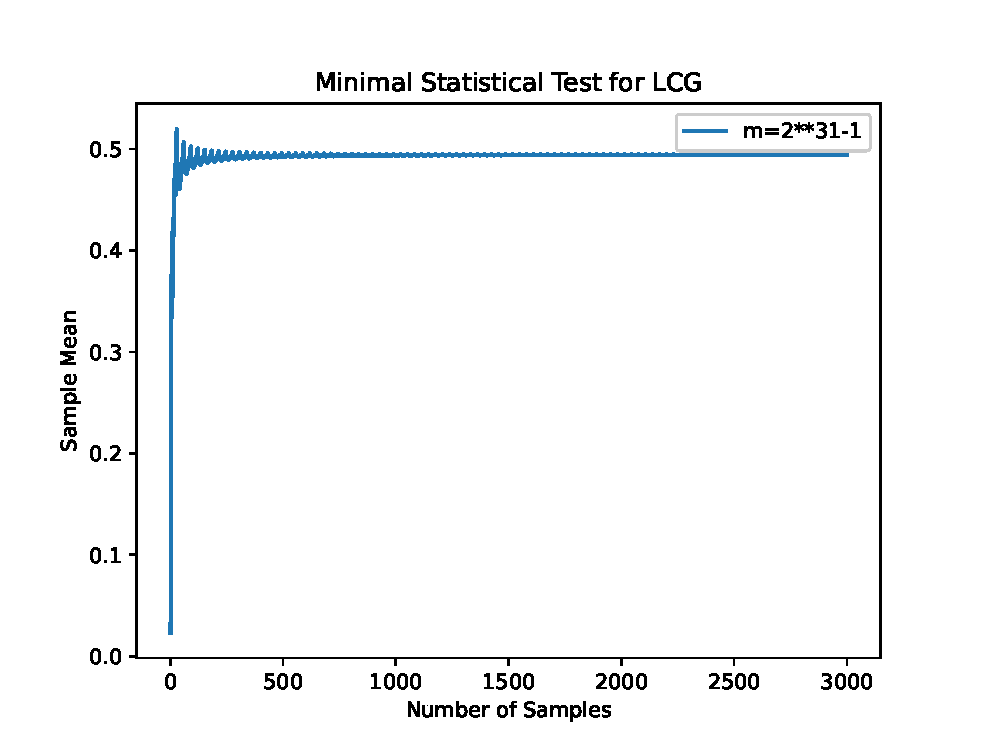
\includegraphics[width=1.1\textwidth]{Problem_1.1}
            \caption{\fontsize{10pt}{15pt}\selectfont 种子值取12345678时,最后收敛到0.5左右,“成功”复现图像}
        \end{minipage}\label{fig:figure2}
    \end{figure}

    通过调整种子值的大小我们可以控制最终随机数的期望,但是按照随机数的要求,我们不应该令随机数的期望与种子值有关(至少应维持在0.5左右)。
    所以我对该组参数的选取持质疑态度,在后面问题解答中我将提出我的看法。

    \subsection{问题二阐述}
    当参数为$m=27,a=26,c=5$时,我们先选取种子值为$x_0=4$得到Figure 4,再选取种子值为$x_0=6$得到Figure 5.

    \begin{figure}[H]% 插入两张图片并且并排
        \centering
        \begin{minipage}{0.48\textwidth}
            \centering
            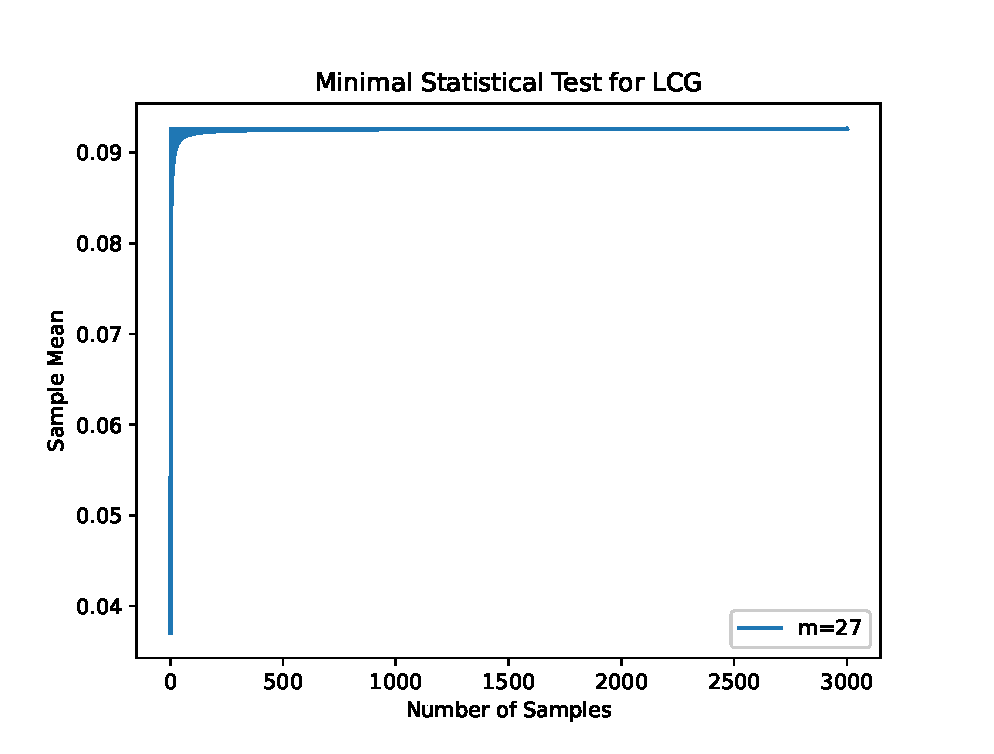
\includegraphics[width=1.1\textwidth]{Problem_2.1}
            \caption{\fontsize{10pt}{15pt}\selectfont 种子值取4时,期望收敛到0.1左右}
        \end{minipage}
        \hspace{0cm}% 图片间距
        \hfill% 撑满整行
        \begin{minipage}{0.48\textwidth}
            \centering
            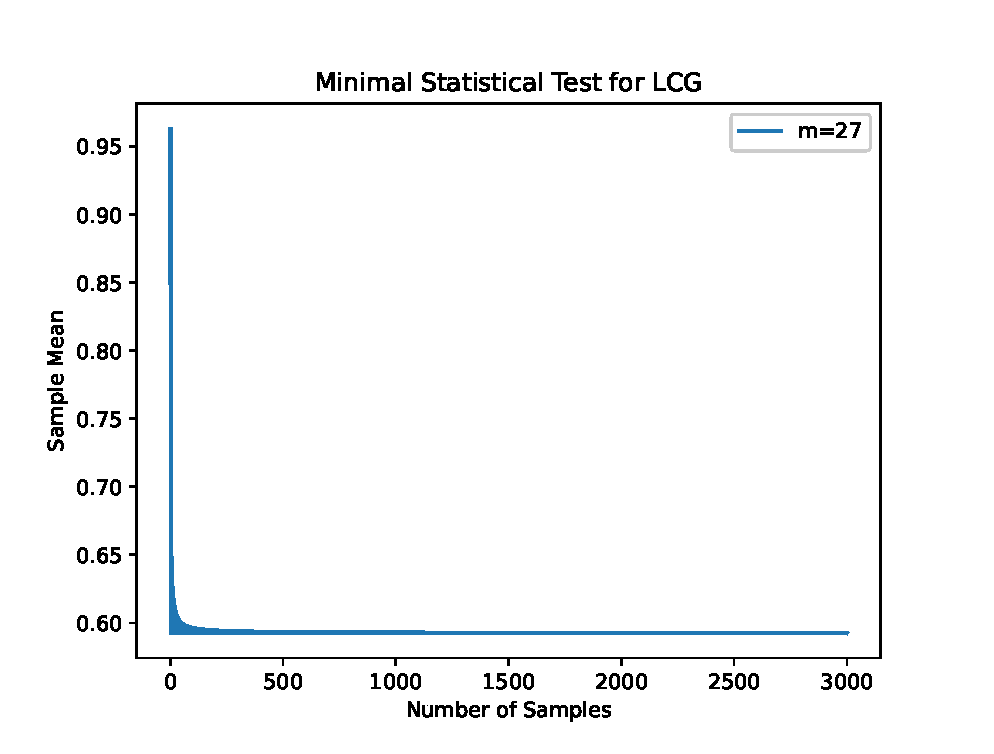
\includegraphics[width=1.1\textwidth]{Problem_2.2}
            \caption{\fontsize{10pt}{15pt}\selectfont 种子值取6时,期望收敛到0.6左右}
        \end{minipage}\label{fig:figure3}
    \end{figure}

    后续我们选取不同种子值,发现在$x_0\leq 5$时,最终期望均收敛到0.1左右,而对于$x_0 > 5$时,最终期望值均收敛到0.6左右,
    不管如何改变种子值的选取,我们都发现该组参数下的期望值始终不会趋于0.5左右,无法复现题目中要求的图像。


    \section{问题解答}
    针对上述两个问题,我不得不从数学角度思考线性同余本身的一些特性,希望能够从中得出问题的解答。

    \subsection{数学求解}
    首先,我们可以先不考虑递推关系后的取余运算,而是直接先根据递推关系求得通项公式再取余运算,证明如下:

    设$x_n=x'+d*m$,其中$x'$是$x_n$模$m$后的余数,d是整数,根据递推关系,
    \[x_n = (ax_{n-1}+c)    (mod M) \]
    代入后得:
    \[x_n = (a(x_{n-1}^{'}+d*m))(mod M)\]

    在取余运算中$a*d*m$项被约去,所以先代入通项公式再取模与先取模再代入递推关系得到的结果是一样的。

    所以线性同余递推关系可改写为:
    \begin{equation}
        x_{n+1}=a^n(x_0+\frac{c}{a-1})-\frac{c}{a-1}
    \end{equation}

    不难判断:


    1)如果某LCG产生的随机序列的周期T小于m,则选取不同的初始值$x_0$产生的LCS(
    Linear Congruential Scquence;线性同余序列
    )可能有不同的周期。

    2)如果其周期T=m,则即使选取不同的$x_0$,产生的这些LCS具有相同的周期且必定为T。


    下列定理给出了混合同余发生器达到满周期的一个充分条件:
    \begin{theorem}
        当下列三个条件都满足时,混合同余发生器可以达到满周期:

        \hspace{2cm}(1)c与M互素;

        \hspace{2cm}(2)对M的任一个素因子P,a-1被P整除

        \hspace{2cm}(3)如果4是M的因子,则a-1被4整除。
    \end{theorem}

    我们常取$M=2^L$,$L$是计算机中整数的尾数字长。按照上述定理的建议可取$a=4\alpha+1,c=2\beta+1$,$\alpha,\beta$为任意正整数。$x_0$为任意非负整数,这样的LCG是满周期的,周期为$2^L$.

    好的均匀分布随机数发生器应该周期足够长,统计性质符合均匀分布,序列之间独立性好。把同余法生成的数列看成随机变量序列$\{x_n\}$,在满周期时,可认为$x_n$是从$0\sim M-1$中随机等可能选取的,即
    \[P\{x_n=i\}=1/M,i=0,1,\ldots,M-1\]
    此时
    \[E\left( x_n \right)=\sum_{i=0}^{M-1}i\cdot\frac{1}{M}=(M-1)/2\]
    \[S^2 \left( x_n \right)=E\left( x_n^2 \right)-\left( E\left( x_n \right) \right)^2 =\sum^{M-1}_{i=0}i^2\frac{1}{M}-\frac{\left( M-1 \right)^2}{4}=\frac{1}{12}\left( M^2-1 \right)\]
    于是当M很大时,
    \[E\left( x_n \right)=\frac{1}{2}-\frac{1}{2M}\approx \frac{1}{2}\]
    \[S^2 \left( x_n \right)=\frac{1}{12}-\frac{1}{12M^2}\approx\frac{1}{12}\]

    可见M充分大时从一、二阶矩看生成的数列很接近均匀分布。

    随机数序列还需要有很好的随机性。数列的排列不应该有规律,序列中的两项不应该有相关性。


    因为序列由确定性公式生成,所以不可能真正独立。至少我们要求是序列自相关性弱。对于满周期的混合同余发生器可以得序列中前后两项自相关系数的近似公式
    \[\rho\left( 1 \right)\approx \frac{1}{a}-\frac{6c}{aM}\left( 1-\frac{c}{M} \right)\]

    所以应该选取较大a值。

    \subsection{问题求解}
    回到问题中来,问题一、二之所以与种子值相关,均是因为其并没有达到满周期,由于糟糕的a的取值,导致LCS的周期较小(比方说问题二的T只有2),最后的序列期望与均匀分布的期望相差甚远。

    我们可以更改问题一中的取值,使用C++11中的随机数参数$a=16807$,种子数随机选取,得到的期望图像见Figure 6.
    \begin{figure}[htbp]
        \centering
        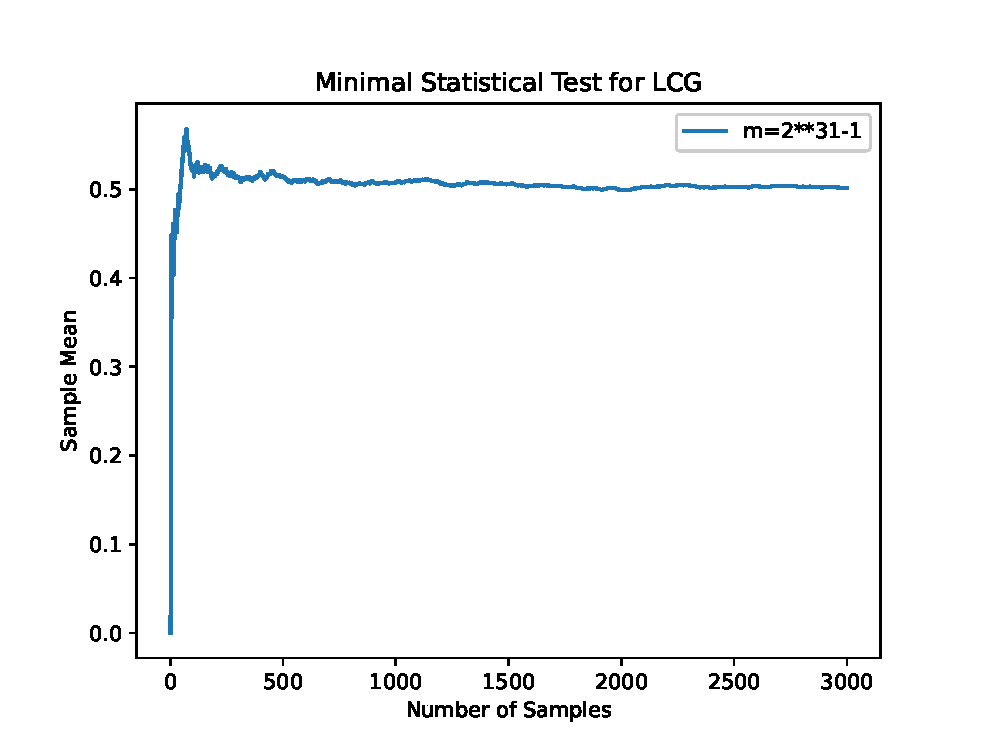
\includegraphics[height=8cm]{Problem_3}\label{fig:figure4}
        \caption{参数$a=16087,x_0=1$}
    \end{figure}

    改变参数a后其期望趋近于0.5左右,与均匀分布的期望接近。


    \section{总结}

    简单总结几点即是:

    1)模数m应该尽可能大,通常至少大于$2^{30}$,为了计算效率,通常会结合计算机的字长考虑选取m的值。

    2)如果m选取为2的幂,也即$m=2^l$,则选取的a通常应该满足a模8等于5。

    3)当参数m和a的选定比较合理时,对于c的选择约束性不是很强烈,但要保证c与m互质。例如c可以选择1或者11。

    4)种子seed应该是随机选取的,可以将时间戳作为种子。


\end{document}% 结束文档编辑,后面写啥都编译不出来
